% !TeX spellcheck = en_US
\documentclass[a4paper]{report}
\usepackage[T1]{fontenc}
\usepackage[utf8]{inputenc}
\usepackage[english]{babel}
\usepackage{geometry}
\usepackage{graphicx}
\usepackage{subfig}
\usepackage{lipsum}
 \geometry{a4paper,top=2.5cm,bottom=2.5cm,left=3cm,right=3cm,%
	heightrounded,bindingoffset=5mm}

\usepackage{color}
\usepackage{listings}
\usepackage{xcolor}

\colorlet{punct}{red!60!black}
\definecolor{background}{HTML}{EEEEEE}
\definecolor{delim}{RGB}{20,105,176}
\colorlet{numb}{magenta!60!black}

\lstset{ %
	language=C++,                % choose the language of the code
	basicstyle=\footnotesize,       % the size of the fonts that are used for the code
	numbers=left,                   % where to put the line-numbers
	numberstyle=\footnotesize,      % the size of the fonts that are used for the line-numbers
	stepnumber=1,                   % the step between two line-numbers. If it is 1 each line will be numbered
	numbersep=5pt,                  % how far the line-numbers are from the code
	backgroundcolor=\color{white},  % choose the background color. You must add \usepackage{color}
	showspaces=false,               % show spaces adding particular underscores
	showstringspaces=false,         % underline spaces within strings
	showtabs=false,                 % show tabs within strings adding particular underscores
	frame=single,           % adds a frame around the code
	tabsize=2,          % sets default tabsize to 2 spaces
	captionpos=b,           % sets the caption-position to bottom
	breaklines=true,        % sets automatic line breaking
	breakatwhitespace=false,    % sets if automatic breaks should only happen at whitespace
	escapeinside={\%*}{*)}          % if you want to add a comment within your code
}

\lstdefinelanguage{json}{
	basicstyle=\normalfont\ttfamily,
	numbers=left,
	numberstyle=\scriptsize,
	stepnumber=1,
	numbersep=8pt,
	showstringspaces=false,
	breaklines=true,
	frame=lines,
	backgroundcolor=\color{background},
	literate=
	*{:}{{{\color{punct}{:}}}}{1}
	{,}{{{\color{punct}{,}}}}{1}
	{\{}{{{\color{delim}{\{}}}}{1}
	{\}}{{{\color{delim}{\}}}}}{1}
	{[}{{{\color{delim}{[}}}}{1}
	{]}{{{\color{delim}{]}}}}{1},
}

%{0}{{{\color{numb}0}}}{1}
%{1}{{{\color{numb}1}}}{1}
%{2}{{{\color{numb}2}}}{1}
%{3}{{{\color{numb}3}}}{1}
%{4}{{{\color{numb}4}}}{1}
%{5}{{{\color{numb}5}}}{1}
%{6}{{{\color{numb}6}}}{1}
%{7}{{{\color{numb}7}}}{1}
%{8}{{{\color{numb}8}}}{1}
%{9}{{{\color{numb}9}}}{1}

\newcommand{\HRule}{\rule{\linewidth}{0.5mm}}

\begin{document}
\begin{titlepage}
	\begin{center}
		
		% Top 
		
\includegraphics[width=0.45\textwidth]{img/unipi.png}~\\[2.5cm]
		
		
		% Title
		\HRule \\[0.4cm]
		{ \LARGE 
			\textbf{JustRecipe}\\[0.4cm]
			\emph{Group Project for Large Scale and Multi-Structured Databases}\\[0.4cm]
		}
		\HRule \\[1.5cm]
		
		
		
		% Author
		{ \large
			Francesco Campilongo \\[0.1cm]
			Daniele Cioffo \\[0.1cm]
			Francesco Iemma \\[0.1cm]
		}
		
		\vfill

		%\textsc{\large Department of Electrical Engineering,\\Computer Engineering \& Informatics}\\[0.4cm]
		
		
		% Bottom
		{\large Academic Year 2020/21}
		
	\end{center}
\end{titlepage}


\tableofcontents

\chapter*{Introduction}
In the social network era the large scale databases topic is very relevant. The handling of big data such as informations of users and moreover is a critical asset of our society. In fact, from the viewpoint of the security is very important to handle in the correct way this very huge amount of data because, otherwise, it is possible to have leak of critical information that cause critical issues about users privacy.

\noindent Another problem caused from large amount of data created from the applications used every day from all of us, is the following: \emph{How we can manage this data?}.

\noindent Nowadays we have a lot of tools to do this, the most famous, and maybe the most used, is for sure MongoDB. It allows us to handle a huge amount of data without critical issues and maintaining good performance. Another well-known tool is Neo4J (and so Graph DB) that is in charge of handle the social part of the application, in fact the graph is indeed a network, and so this is the best way to represents a social network where the interactions between users are fundamental and very widespread.

\noindent Our aim is to design and implement a modern application which can handle a huge amount of data maintaining good performance and implementing a social network side in order to exploit the desire for social relations of our society.



\chapter{Dataset}
In this first chapter of this document we will talk about searching for the initial dataset.

\noindent As specified in the project documentation, the dataset had to be at least 50MB large, and this quantity could not be generated directly within the application. So we did an initial search, finding two datasets, which were generated by their authors by performing the scraping on the sites \emph{www.FoodNetwork.com} and \emph{www.Epicurios.com}. The second dataset was more complete (more nutritional values), so it was used as the main dataset. The other dataset was used to complement the other, reaching a total of  67.8 MB, with 45349 recipes.

\noindent To correctly extract the data present in the two datasets we wrote a program in Java, called \emph{RecipeReade}r, thanks to which we adapted the two different formats and removed the duplicates (recipes with the same title that were present in both datasets).
To implement this program we used the GSon library and the Jackson library.

\noindent The variety property is ensured by using two different sources. The velocity / variability properties are ensured because comments and recipes are eliminated and added inside the application, indeed this data may lose importance after a certain time interval since new data quickly arrives.

\chapter{Design}
\section{Introduction To The Application}
The topic of cuisine is extensively widespread in our society. In fact we can think at the success achieved by tv shows related to cooking in the last years and also at the fact that a lot of chefs are becoming superstars.
Then there is another important factor: the coronavirus outbreak.

\noindent With the coronavirus outbreak a lot of people became cuisine lovers, in fact at the first moments of the pandemia several ingredients as flour and yeast were very hard to find, because people were confined in their home and so they had more free time.

\noindent But this topic is not a recente one. The first recipe book dates back to eigth century B.C. and it is the so-called \emph{Eraclio} (by the name of the city in which he was found). Then also an important latin writer, Apicio, wrote one of the most important recipe books of the roman era: \emph{De Re Coquinaria} which dates back to the first century B.C..
 
\noindent So the topic of cuisine is inherent to human nature, because the necessity of eating is a basic need.
Furthermore, everyone has experimented the infamous question: “What will I eat this evening?”. JustRecipe has the aim of answer to this question, it has the aim of helping university student or workers to retrieve and to do fast and simple recipes.

\noindent So this application is basically a recipe book but it is also more than this.

\noindent JustRecipe is also a social network which allow people to enjoy, to ex-change ideas about cooking, to feel less lonely in this hard period.

\section{Requirements}
\subsection{Main Actors}
The main actors of the application are four:
\begin{itemize}
	\item Unregistered User
	
	\noindent He is the user which open the application for the first time, in order to access he must sign-up.
	
	\item User
	
	\noindent He is the normal user (the registered one).
	
	\item Moderator
	
	\noindent He is in charge of controlling the comments and eventually delete the ones which contain abuses.
	
	\item Administrator
	
	\noindent He is the most powerful actor, he can delete users and recipes and he is also in charge of elect moderators
\end{itemize}

\noindent Each actor can do all the features of the previous ones in the list.

\subsection{Functional Requirements}
\subsubsection{Features offered to the Unregistered User}
\begin{itemize}
	\item  Registration
	
	\noindent In order to access the application an user must sign-up. Otherwise he is not allowed to access and to use all the functionalities.
\end{itemize}
\subsubsection{Features offered to the Registered User}
\begin{itemize}
	\item Login/Logout
	
	\noindent The only way to access the application, as we said previously, is to sign-up and login. At the end the user can logout and close the session.
	
	\item Search a recipe
	
	\noindent It's possible to search a recipe searching for the title and for categories.
	
	\item Browse suggested recipes
	
	\noindent The suggestions will be offered in a proper section, they are done considering the relationships between the user logged, the users followed by the user logged and so on so forth.
	
	\item Browse recipes of following users
	
	\noindent In a proper section (i.e. the Homepage) the user can browse the recipes of the following user. Indeed he can see only a snapshot of the recipes. If he wants a more in-depth view, he can click on it and see the recipe page in which he is able to see all the recipe details. 
	
	\item Add a recipe
	
	\noindent The user can insert a new recipe.
	
	\item Edit own recipes
	
	\noindent The user can edit the recipes previously added by himself.
	
	\item Comment recipes
	
	\noindent
	Every user can make a comment about recipes
	
	\item Follow another user
	
	\noindent The most important feature of each social network: the users can follow each others. 
	
	
	\item Like a recipe
	
	\noindent In order to evaluate a recipe each user can like its.
\end{itemize}

\subsubsection{Features offered to the Moderator}
\begin{itemize}
	\item Delete comments
	
	\noindent The moderator is in charge of delete comments which contain racist abuse, crude terms and so on so forth.
\end{itemize}

\subsubsection{Features offered to the Administrator}
\begin{itemize}
	\item Delete users
	
	\noindent The admin can delete the users which don't respect the application guidelines.
	
	\item Delete recipes
	
	\noindent The admin can delete recipes not correctly inserted
	
	\item Elect moderators
	
	\noindent In order to handle better the application, the admin can elect some users as moderators.
\end{itemize}
\subsection{Non-Functional Requirements}
The non-functional requirements of the applications are described in the following lists:
\begin{itemize}
	\item \emph{usability}
	\item \emph{data availability}
	\item \emph{Tolerance to single point of failure}: if a server crashes another one is available (thanks to replicas). Parlare quindi dell'eventual consistency.
	\item \emph{dire qualcosa sulla sharding}
	\item \emph{Reliability}
	\item \emph{Security and data encryption???}
\end{itemize}
\newpage
\subsection{Actors and Use Cases}
The use case diagram of the application is described in the figure 2.1

\begin{figure}[htpb]
	\centering
	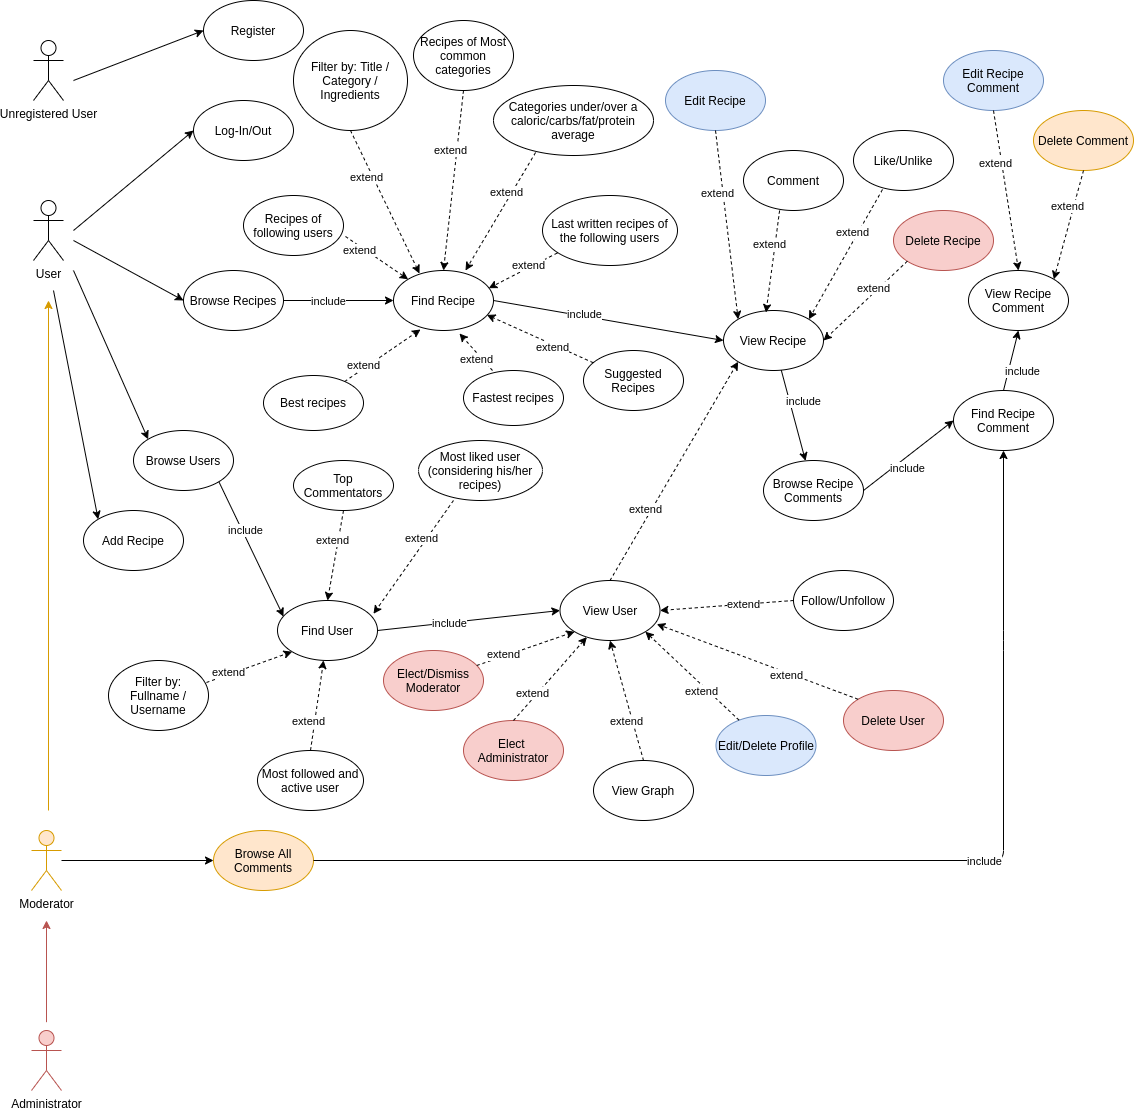
\includegraphics[scale=0.4]{img/UseCaseDiagram.png}
	\caption{Use Case Diagram}
\end{figure}

\noindent Some observations on the diagram are necessary:
\begin{itemize}
	\item The circles in \underline{blue} are the ones which described actions available only for the owner of the object on which the actions are applied.
	
	\noindent So, in detail, this means that a \textbf{User} can edit/delete a profile if and only if he owns this profile. Then he can edit a recipe and/or a comment if and only if he adds that recipe or that comment.
	
	\item When we are seeing the recipe detail we can go on the user that have been added that recipe. So the extend relation between \emph{View Recipe} and \emph{View User} means this.
	
	\item The action \emph{Browse Recipes of following users} is available only if the \textbf{User} follows at least one user. Otherwise he can start to follow users and only after this he can see suggested recipes (\emph{Browse Suggested Recipes}). In this case, due to the fact that the user follows nobody, he will see the most famous recipes in general because it's impossible to suggest specific recipes due to the fact that he has no following and no likes or comments. 
	
	\item The actions in \underline{red} are the ones that can be performed only by the \textbf{Administrator}
	
	\item The actions in \underline{orange} are the ones that can be performed only by the \textbf{Moderators}
\end{itemize}


\section{UML Class Diagram}
Let analyze the UML Class Diagram. There are three main entities: User, Comment, Recipe.

\noindent It's important to point out that the \textbf{User} of the Use Case Diagram is here the so-called \emph{Registered User} and the \emph{User} of this diagram is the generic user. Then we undeline the fact that, in order to represent the three actors of the use case diagram, a generalization is needed.
 
\begin{figure}[htpb]
	\centering
	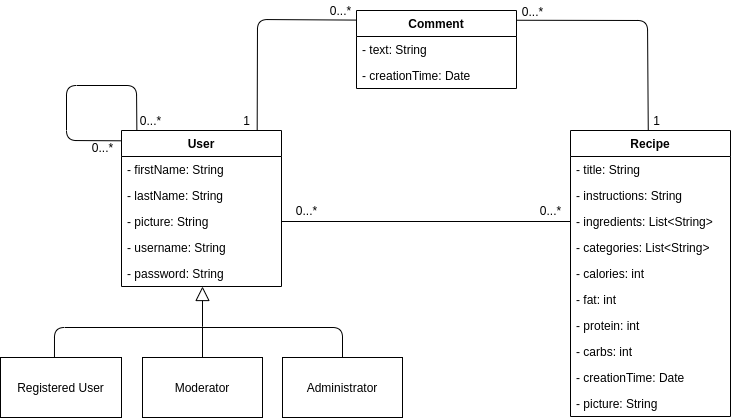
\includegraphics[scale=0.5]{img/ClassDiagram_generaliz.png}
	\caption{UML Analysis Classes Diagram with generalization unsolved}
\end{figure}

\noindent Observing the figure 2.2 it's possible to understand that we can resolve the generalization putting an attribute in the entity \emph{User}. It is an integer and we call it \emph{role}: if it's a \emph{Normal User} role is 0; if \emph{Moderator} then 1; if \emph{Administrator} then 2.

\begin{figure}[htpb]
	\centering
	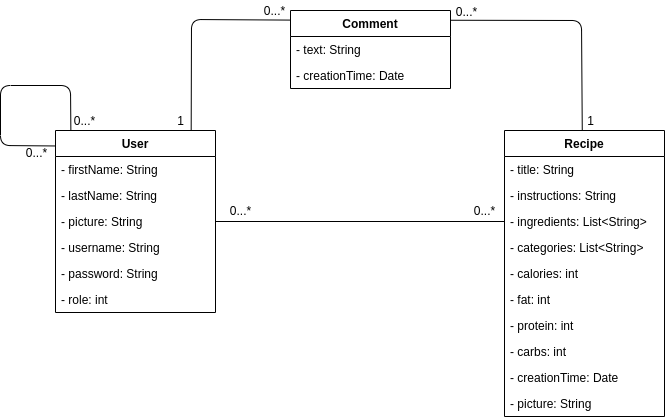
\includegraphics[scale=0.5]{img/ClassDiagram.png}
	\caption{UML Analysis Classes Diagram}
\end{figure}

\newpage
\subsubsection{Classes definitions}
Classes definitions:
\begin{table}[ht]
\caption{Classes definitions} % title of Table
\centering % used for centering table
\begin{tabular}{c c} % centered columns (2 columns)
\hline\hline %inserts double horizontal lines
Class & Description \\ [0.5ex] % inserts table
%heading
\hline % inserts single horizontal line
Registered User &  A standard user (registered one) who can only perform basic operations \\
Moderator & User who can also check comments and decide to delete them  \\ 
Administrator & Most powerful user, he can also delete users and recipes, and elect moderator \\
Comment & Comment posted by a user \\
Recipe & Recipe added by one user  \\ [1ex] % [1ex] adds vertical space 
\hline %inserts single line
\end{tabular}
\label{table:classes definitions} % is used to refer this table in the text
\end{table}

\subsubsection{Classes attributes}
Classes attributes:
\begin{table}[ht]
\caption{Classes attributes - User}
\centering 
\begin{tabular}{c c c}
\hline\hline
Attribute & Type &  Description \\ [0.5ex]
\hline 
firstName & String &  First name of the user \\
lastName & String & Last name of the user  \\ 
picture & String &  URL of the profile picture \\
username & String & Username of the user (identifier) \\
password & String & Password chosen by the user, used for the login phase  \\ 
role & int & Role of the user (0: Normal User, 1: Moderator, 2: Administrator)\\[1ex] 
\hline 
\end{tabular}
\end{table}

\begin{table}[ht]
\caption{Classes attributes - Comment}
\centering 
\begin{tabular}{c c c}
\hline\hline
Attribute & Type &  Description \\ [0.5ex]
\hline 
text & String &  Plain text of the comment \\
creationTime & Date & Creation timestamp of the comment  \\[1ex] 
\hline 
\end{tabular}
\end{table}

\begin{table}[ht]
\caption{Classes attributes - Recipe}
\centering 
\begin{tabular}{c c c}
\hline\hline
Attribute & Type &  Description \\ [0.5ex]
\hline 
title & String &  Title of the recipe (identifier) \\
instructions & String & Operations to be performed to make the recipe  \\ 
ingredients & List<String> &  Ingredients to be used in the recipe \\
categories & List<String> & Categories to which the recipe belongs \\
calories & int & Calories contained in the recipe  \\ 
fat & int & Fat contained in the recipe  \\ 
protein & int & Protein contained in the recipe  \\ 
carbs & int & Carbs contained in the recipe  \\ 
creationTime & Date & Creation timestamp of the recipe \\
picture & String & URL of the recipe picture \\[1ex] 
\hline 
\end{tabular}
\end{table}

\section{Data Model}
In this section we will discuss about the design choises performed in terms of data model and the databases used in order to handle in the better way our dataset.
\subsection{DocumentDB}
The document DB is used in order to handle the large dataset of recipes that we have. In particular, MongoDB allow us to perform fast query even if the size of the dataset is very big and this is the main reason that brings us to choose it. Moreover it is schemaless and this allow us to maintain etherogenous recipes in our database (some recipes have some attributes, instead others have not those). 
\lstset{ language=json}
\begin{lstlisting}
{
	"_id":
			{"$oid": "5fdb5fd86796ee4e73ef5b84"},
	"title": 
			"Lentil, Apple, and Turkey Wrap ",
	"instructions": 
			"1. Place the stock, lentils, celery, carrot, thyme, and
			salt in a medium saucepan and bring to a boil. Reduce heat
			to low and simmer until the lentils are tender, about 30
			minutes, depending on the lentils. (If they begin to
			dry out, add water as needed)..." ,
	"ingredients":
			["4 cups low-sodium vegetable or chicken stock", "1 cup dried brown lentils", ...],
	"categories":
			["Sandwich", "Bean", "Fruit", "Tomato", "turkey", ...],
	"calories":
			426,
	"fat":
			7,
	"protein":
			30,
	"carbs":
			20,
	"creationTime":
			{
				"$date": "2020-12-17T13:40:40.658Z"
			},
	"authorUsername":
			"oscar.evans",
	"picture":
			"https://assets.epicurious.com/photos/551b0595e7851a541a30b23f/master/pass/239173_lentil-apple-and-turkey-wrap_6x4.jpg",
	"comments":
			[
				{
					"authorUsername": "oliver.smith",
					"text": "Very good!!!",
					"creationTime":
					{
						"$date": "2020-12-17T13:50:40.658Z"
					}
				},
				{
					"authorUsername": "jessica.evans",
					"text": "Fantastic",
					"creationTime":
					{
						"$date": "2020-12-17T13:52:40.658Z"
					}
				},....
			]
}
\end{lstlisting}  
\subsection{GraphDB}
The Graph database is the one that handles the social part of the application. Thanks to it we are able to analyze the relationships among users and their recipes. The graph database that we use is Neo4J.

\noindent We have two type of nodes within the database:
\begin{itemize}
	\item \textbf{User}: it is the node that represents the user inside the graph. Its attribute are: \emph{firstName}, \emph{lastName}, \emph{username}, \emph{password}, \emph{picture}\footnote{Only the URL of the picture is saved in this field, otherwise the size of this attribute would be too large}, \emph{role}\footnote{0 for the normal user, 1 for moderator and 2 for the administrator}.
	
	\item \textbf{Recipe}: it is the node that represents the recipe within the graph. Its attribute are: \emph{title}, \emph{calories}, \emph{fat}, \emph{carbs}, \emph{protein}, \emph{picture}$^1$
\end{itemize}

\noindent The information about the user are present only on Neo4J because we handle the social part only with it. Instead some information about recipes are present in both databases, in particular on Neo4J we have info that are already present also in MongoDB, but the opposite is not true.

\noindent The Neo4J relationships are:
\begin{itemize}
	\item \textbf{Adds}: if the user \emph{A} has added the recipe \emph{R}, then we have a relationship \emph{:ADDS} from \emph{A} to \emph{R} ($A \rightarrow R$).
	
	\noindent We have as property, the one called \emph{when} that is the timestamp which indicates when the recipe has been added.
	
	\item \textbf{Follows}: if the user \emph{A} has followed the user \emph{B}, then we have a relationship \emph{:FOLLOWS} from \emph{A} to \emph{B} ($A \rightarrow B$).
	
	\item \textbf{Likes}: if the user \emph{A} has liked the recipe \emph{R}, then we have a relationship \emph{:LIKES} from \emph{A} to \emph{R} ($A \rightarrow R$).
\end{itemize}  

\noindent All the relationships that starts from a node \emph{X} are deleted if \emph{X} has deleted, furthermore if \emph{X} is a user, also the recipes that he has added will be eliminated. In figure 2.4 we can see an example of the nodes, the relationships and the attributes.

\begin{figure}[htpb]
	\centering
	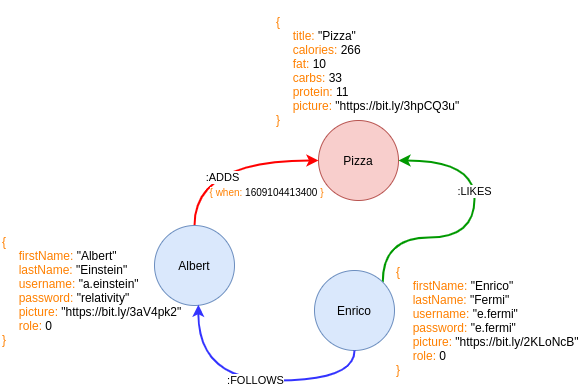
\includegraphics[scale=0.6]{img/graphDbModel.png}
	\caption{Example of Neo4J nodes and relationships}
\end{figure}

\section{Distributed Database Design}
\subsection{Replicas}
\subsection{Sharding}
\section{Software Architecture}


\chapter{Implementation and Test}
\section{Main Modules}
The implementation code is divided into two main modules: RecipeReader and JustRecipe.
 \begin{itemize}
	\item \emph{RecipeReader}:  is a program we wrote to get our initial dataset, extracting the information that interests us from the two initial datasets (see chapter 1). 
	\item \emph{JustRecipe}:  is the actual application, whose implementation will be analyzed in more detail in the next sections. The application was developed following the MVC (Model, View, Controller) pattern. The View displays the data contained in the model and was mainly developed using .fxml files, which allow you to write all the graphic components and their properties in separate files. The Model provides methods for accessing data useful for the application. The Controller receives the commands from the user and implements them by changing the status of the other two components. This division allowed us to completely separate the three components, for a more readable and maintainable code.
\end{itemize}
\section{Main Packages and Classes}
In this section will be presented the main packages of JustRecipe module and the respective classes.
\subsection {it.unipi.dii.inginf.lsdb.justrecipe.config}
This package is used to handle the configuration parameters, stored in \emph{config.xml}. The schema for the validation is in the file \emph{config.xsd}. The validation is very important to be sure of the correctness of the file \emph{config.xml}.

\noindent Classes:
 \begin{itemize}
	\item \emph{ConfigurationParameters}: this class store all the configuration parameters needed by the application. For example the IP for the Neo4j database. These values do not need to be changed, so only get methods are provided. 
\end{itemize}
\subsection {it.unipi.dii.inginf.lsdb.justrecipe.main}
This package contains the Main class, that starts the application.

\noindent Classes:
 \begin{itemize}
	\item \emph{Main}: this class extends \emph{Application} and implements the \emph{start} method. 
\end{itemize}
\subsection{it.unipi.dii.inginf.lsdb.justrecipe.model}
This package contains the classes required for the model. These classes are the java bean for our application.

\noindent Classes:
  \begin{itemize}
	\item \emph{Comment}: This class stores all the information about a comment, like the text, the username of the author and the timestamp of creation. 
	\item \emph{Recipe}: This class stores all the information about a recipe, like the title, the ingredients, and so on.
	\item \emph{User}: This class stores all the information about a user, like the username, the password, and so on.
	\item \emph{Session}: This class is used to maintain the information of the session, like the logged user. We used the singleton design pattern for this class.
\end{itemize}
\subsection {it.unipi.dii.inginf.lsdb.justrecipe.persistence}
This package deals with managing the persistence of data, in fact it contains the classes used to interface with databases.

\noindent Classes:
 \begin{itemize}
	\item \emph{DatabaseDriver}: this \emph{interface} declares all the methods that has to be implemented in a database driver. This methods are \emph{initConnection()} and \emph{closeConnection()}.  
	\item \emph{MongoDBDriver}: this class implements DatabaseDriver and is responsible for implementing all the queries that have to be run on MongoDB. We used the Singleton design pattern, because a single instance of this driver must be shared by all application classes.
	\item \emph{Neo4jDriver}: this class implements DatabaseDriver and is responsible for implementing all the queries that have to be run on Neo4j. We used the Singleton design pattern, because a single instance of this driver must be shared by all application classes.
\end{itemize}
\subsection {it.unipi.dii.inginf.lsdb.justrecipe.controller}
This package contains the classes required for the controller part of the MVC pattern. For each different page to be shown to the user, a special controller has been implemented, which manages the events resulting from the actions taken by the user and updates the model and the view.

\noindent Classes:
 \begin{itemize}
	\item \emph{WelcomePageController}: this class manages the login/register page of the application.
	\item \emph{HomePageController}: this class handles the homepage section of the application (shows the recipes of following users and handles the event, like the click on a recipe snapshot).
	\item \emph{DiscoveryPageController}: this class manages the discovery section of the application. So it is in charge of showing the results of search made by the user.
	\item \emph{ProfilePageController}: this class manages the profile section of the application. The profile could be either mine or someone else's. Thanks to this class it is possible to manage some events such as following a user, deleting my profile, seeing his recipes, and so on.
	\item \emph{AdministrationPageController}: this class handles the Administration section of the application. Of course, not all the users can access to this page, only the moderator (for seeing the last comments) and the administrators (for doing all the possible operations) can access.
	\item \emph{EditProfilPageController}: this class manages the page for editing the personal profile. The user can insert a new profile image, change the personal information, and so on. The administrator can change the role of the user in this page.
	\item \emph{AddRecipePageController}: this class manages the page of the application used for insert a new recipe. 
	\item \emph{RecipeSnapshotController}: this class manages the single recipe snapshot, like the click on him.
	\item \emph{RecipePageController}: this class handles the page in which we show all the information about a recipe. In this page it is possible also to comment a recipe and see the comments already done.
	\item \emph{CommentController}: this class manages the single comment and all the operations that can be done on him.
	\item \emph{UserSnapshotController}: this class manages the single snapshot of one user, and all the operations that can be done on him.
\end{itemize}
\subsection {it.unipi.dii.inginf.lsdb.justrecipe.utils}
This package contains a class used to store all the utility functions that we use in the application.

\noindent Classes:
 \begin{itemize}
	\item \emph{Utils}: this class is used to contain some utility functions used inside the application (to avoid replicating parts of code).
\end{itemize}
\section{Most Relevant Queries}
In the following section will be presented the most relevant query performed with MongoDB and Neo4J. 
\noindent Some important point must be underlined:
\begin{itemize}
	\item The operation of \emph{skip} and \emph{limit}, use in the most of the following queries, are necessary due  to implementation reasons. In fact the results are not shown all in the same page (because of the size of the database the output can be huge) but only a subset of the result are shown (for instance, the first X) and in order to go on and see the other result, the query will be performed with different value of \emph{<howManyToSkip>} (the first time is 0, the second is X) and \emph{<howManyToGet>} (it's a fixed number, must be equal to the previous X)
	\item In Neo4J part, due to performance reasons, some queries compute also followers, followings and recipes added by each user. This is necessary because when the user is given as result this information must be showed and if we don't compute it here we have to do another query for each user.
\end{itemize}

\subsection{MongoDB}

\subsubsection{Recipes of the user}

This query gives the opportunity to collect all the recipes written by a specific User through checking the author username field. This search is case sensitive cause we are using the username.
\begin{itemize}
	\item Input: a string who rapresent an username (unique through the users), how many recipe to skip, and how many to get.
	\item Output: a list of recipes, all added by the user erlier selected, ordered by the .
\end{itemize}
\lstset{ language=C++}
\begin{lstlisting}
db.recipes.aggregate (
	[
		{ 
			$match : 
			{ 
				authorUsername: <authorUsername>
			}  
		},
		{ 
				$sort : 
			{ 
				creationTime : -1 
			} 
		},
		{ 
			$skip: <howManyToSkip> 
		},
		{ 
			$limit: <howManyToGet> 
		}	
		]
)
\end{lstlisting}
\subsubsection{Search for recipe title}
Given a portion of the title, this query is capable of returning as a result a set of recipes whose titles contain it. Research must be case insensitive (see \emph{options:"i"} in the regexMatch step of the aggregation)
\begin{itemize}
\item Input: portion of the title, how many recipes to skip and how many recipes to get.
\item Output: set of recipes.	
\end{itemize}
\lstset{ language=java}
\begin{lstlisting}
db.recipes.aggregate (
	[
		{ 
			$match : 
			{ 
				title: 
				{
					$regex: /^.*<portionOfTheTitle>.*$/,
					$options: "i"
				} 
			}  
		},
		{ 
			$sort : 
			{ 
				creationTime : -1 
			} 
		},
		{ 
			$skip: <howManyToSkip> 
		},
		{ 
			$limit: <howManyToGet> 
		}	
	]
)
\end{lstlisting} 
\subsubsection{Search for recipe category}
Given the category, or a part of this, the query returns recipes that belong to it. The search is case insensitive.

\noindent It's important to point out that a recipe belongs to more than one categories, so a recipe can be part of the result of the search of two different categories (this is normal and it is allowed). 

\begin{itemize}
	\item Input: portion of the category or the entire one \emph{<portionOfTheCategory>}, how many recipes to skip \emph{<howManyToSkip>} and how many to get \emph{<howManyToGet>}.
	\item Output: set of recipes belonging to the given category
\end{itemize}
\begin{lstlisting}
db.recipes.aggregate (
	[
		{ 
			$match : 
			{ 
				categories: 
				{
					$regex: /^.*<portionOfTheCategory>.*$/,
					$options: "i"
				} 
			}  
		},
	{ 
		$sort : 
		{ 
			creationTime : -1 
		} 
	},
	{ 
		$skip: <howManyToSkip> 
	},
	{ 
		$limit: <howManyToGet> 
	}	
	]
)
\end{lstlisting}

\subsubsection{Search for recipe ingredients}
This query give the possibility to find a specific number of recipes given some of the recipe ingredients. The search is case insensitive for a more easy to use experience.
\begin{itemize}
	\item Input: a list of ingredients, how many recipes to skip and how many recipe to show.
	\item Output: a list of recipes, all of them have at least all the ingredients spicified before. The results are ordered from the newer to the older recipe.
\end{itemize}

\lstset{ language=java}
\begin{lstlisting}
	db.recipes.aggregate (
	[
	{ 
		$match : 
		{ 
			ingredients: 
			{
				$regex: /^.*<ingredients[i]>.*$/,
				$options: "i"
			} 
		}  
	},
	{ 
		$sort : 
		{ 
			creationTime : -1 
		} 
	},
	{ 
		$skip: <howManyToSkip> 
	},
	{ 
		$limit: <howManyToGet> 
	}	
	]
 )
\end{lstlisting} 
\subsubsection{Most common recipe categories}
This query allows you to get a ranking of the categories most used by users for their recipes.
\begin{itemize}
\item Input: how many categories to skip, how many categories to get.
\item Output: list with the categories ordered by the number of use.
\end{itemize}
\lstset{ language=java}
\begin{lstlisting}
db.recipes.aggregate (
	[
		{ 
			$unwind : "$categories" 
		},
		{
			$group :
			{
				_id : "$categories",
			 	numberOfRecipes: 
				{ 
					$sum: 1
				 }
			}
		},
		{
			$project: 
			{
				'category': '$_id',
				numberOfRecipes: 1,
				_id: 0
			}
		},
		{ 
			$sort : 
			{ 
				numberOfRecipes : -1 
			} 
		},
		{ 
			$skip: <howManyToSkip> 
		},
		{ 
			$limit: <howManyToGet> 
		}	
	]
)
\end{lstlisting}

\subsubsection{Recipes with below average calories - TO DO}

\subsubsection{Last Comments}
The query returns the last comments sorted for creation time, in order to have the most recent as first and the most old as last.

\begin{itemize}
	\item Input: \emph{howManyToGet} and \emph{howManyToSkip}
	\item Output: set of the last comments sorted by creation time in descendant order.
\end{itemize}

\begin{lstlisting}
db.recipes.aggregate (
	[
		{ 
			$unwind : "$comments" 
		},
		{ 
			$sort : 
			{ 
				comments.creationTime : -1 
			} 
		},
		{ 
			$skip: <howManyToSkip> 
		},
		{ 
			$limit: <howManyToGet> 
		}	
	]
)
\end{lstlisting}

\subsection{Neo4J}
\emph{Tabella con dominio grafo e descrizione}
\subsubsection{Suggested Recipes - MANCA CODICE}
We have two levels of suggestions with different relevance.
\begin{itemize}
	\item First Level
	
	\noindent Recipe \emph{R} is a first level suggestion for the user \emph{X}, if \emph{R} has been added by the user \emph{Y} where \emph{Y} is followed by \emph{W} who is followed by \emph{X} ($X \rightarrow W \rightarrow Y$). Or \emph{R} has been added by \emph{Z} where \emph{Z} is followed by \emph{Y} ($ X \rightarrow W \rightarrow Y \rightarrow Z$).
	
	\item Second Level
	
	\noindent Recipe \emph{R} is a second level suggestion for the user \emph{X} if \emph{R} has been added by the user \emph{Y} where \emph{Y} is the owner of at least N recipes liked by \emph{X}. 
	
\end{itemize}

\subsubsection{Recipes of following users}
This query returns all the recipes of the following users of a specific user.
\begin{itemize}
	\item Input: How many recipe name to skip, how many recipe name to show and a string who represents a specific username.
	\item Output: A set of recipe name of the specific user's following users have added.
\end{itemize}
\lstset{ language=java}
\begin{lstlisting}
	MATCH (u1:User{username:$username})-[:FOLLOWS]->(u2:User)-[a:ADDS]->(r:Recipe)
	RETURN r.title AS title, r.calories AS calories,
		 r.fat AS fat, r.protein AS protein, r.carbs AS carbs,
		 r.picture AS picture, u2.username AS authorUsername 
	ORDER BY a.when DESC 
	SKIP $skip LIMIT $limit
\end{lstlisting}
\subsubsection{Most followed and active users}
This query returns the list of the most followed and active users, namely the influencers.
Most followed means that the list is ordered by the number of followers.
Active means that the list is ordered by the number of recipes added by the user.
\begin{itemize}
	\item Input: How many users to skip, how many users to show.
	\item Output: A list of the most followed and active users.
\end{itemize}
\lstset{ language=java}
\begin{lstlisting}
	MATCH (u:User)
	OPTIONAL MATCH (u)<-[f1:FOLLOWS]-(:User)
	OPTIONAL MATCH (u)-[f2:FOLLOWS]->(:User)
	OPTIONAL MATCH (u)-[a:ADDS]->(:Recipe)
	RETURN u.firstName, u.lastName, u.username, 
		u.firstName AS firstName, u.lastName AS lastName, 
		u.picture AS picture, u.username AS username,
		u.password AS password, u.role AS role,
	COUNT(DISTINCT f1) AS follower,
	COUNT(DISTINCT f2) AS following,
	COUNT(DISTINCT a) AS numRecipes
	ORDER BY follower DESC, numRecipes DESC
	SKIP $howManySkip LIMIT $howMany
\end{lstlisting}
\subsubsection{Most liked users}
This query returns the list of the most liked users, namely the users who received more like to their recipes.
\begin{itemize}
	\item Input: How many users to skip, how many users to show.
	\item Output: A list of the most liked users.
\end{itemize}
\lstset{ language=java}
\begin{lstlisting}
	MATCH (u:User)
	OPTIONAL MATCH (u)-[:ADDS]->(:Recipe)<-[l:LIKES]-(:User)
	OPTIONAL MATCH (u)<-[f1:FOLLOWS]-(:User)
	OPTIONAL MATCH (u)-[f2:FOLLOWS]->(:User) 
	OPTIONAL MATCH (u)-[a:ADDS]->(:Recipe)
	RETURN u.firstName, u.lastName, u.username, 
		u.firstName AS firstName, u.lastName AS lastName, 
		u.picture AS picture, u.username AS username, 
		u.password AS password, u.role AS role, 
	COUNT(DISTINCT f1) AS follower, 
	COUNT(DISTINCT f2) AS following, 
	COUNT(DISTINCT a) AS numRecipes, 
	COUNT(DISTINCT l) AS totLikes 
	ORDER BY totLikes DESC 
	SKIP $howManySkip LIMIT $howMany
\end{lstlisting}
\subsubsection{Best Recipes}
This query returns the list of the best recipes, namely the most liked ones.
\begin{itemize}
	\item Input: How many recipes to skip, how many recipes to show.
	\item Output: A list of the best recipes.
\end{itemize}
\lstset{ language=java}
\begin{lstlisting}
	MATCH (:User)-[l:LIKES]->(r:Recipe)
	MATCH (u:User)-[:ADDS]->(r)
	RETURN r.title AS title, r.calories AS calories,
		r.fat AS fat, r.protein AS protein, r.carbs AS carbs, 
		r.picture AS picture, u.username AS authorUsername,
	COUNT(DISTINCT l) AS likes 
	ORDER BY likes DESC
	SKIP $skip LIMIT $limit
\end{lstlisting}
To clarify, the first match is used to avoid to consider the recipes which have not at least one like, and the second match is used to find the user that adds the recipe.
\subsubsection{Search for username}
Given a portion of the username, this query is able to return all users whose usernames contain it. The search must be case insensitive, so the toLower function is used. 
\begin{itemize}
\item Input: portion of the username, how many users to skip and how many users to get.
\item Output: set of users.	
\end{itemize}
\lstset{ language=java}
\begin{lstlisting}
	MATCH (u:User)
	WHERE toLower(u.username) CONTAINS toLower($username)
	OPTIONAL MATCH (u)<-[f1:FOLLOWS]-(:User)
	OPTIONAL MATCH (u)-[f2:FOLLOWS]->(:User)
	OPTIONAL MATCH (u)-[a:ADDS]->(:Recipe)
	RETURN u.firstName AS firstName, u.lastName AS lastName, 
		u.picture AS picture, u.username AS username, 
		u.password AS password, u.role AS role, 
	COUNT(DISTINCT f1) AS follower,
	COUNT(DISTINCT f2) AS following, 
	COUNT(DISTINCT a) AS numRecipes
	SKIP $skip LIMIT $limit
\end{lstlisting} 
\subsubsection{Search for user's full-name}
Given the full-name or a part of it, the query returns the users that contains in their full-name the given input. The query is case-insensitive.
\begin{itemize}
	\item Input: The full-name (\emph{\$fullName}), how many users to skip (\emph{\$skip}) and how many users to get (\emph{\$limit}).
	\item Output: The users that contains in their full-name the given input \emph{\$fullName}.
\end{itemize}
\begin{lstlisting}
	 MATCH (u:User) 
	 WHERE
	 toLower(u.firstName+' '+u.lastName)
	 CONTAINS toLower($fullName)
	 OR
	 toLower(u.lastName + ' ' + u.firstName)
	 CONTAINS toLower($fullName)
	 OPTIONAL MATCH (u)<-[f1:FOLLOWS]-(:User)
	 OPTIONAL MATCH (u)-[f2:FOLLOWS]->(:User)
	 OPTIONAL MATCH (u)-[a:ADDS]->(:Recipe)
	 RETURN u.firstName AS firstName, u.lastName AS lastName,
	 	u.picture AS picture, u.username AS username,
	 	u.password AS password, u.role AS role,
	 COUNT (DISTINCT f1) AS follower,
	 COUNT (DISTINCT f2) AS following,
	 COUNT (DISTINCT a) AS numRecipes
	 SKIP $skip LIMIT $limit
\end{lstlisting} 

\section{Tests and Statistical Analysis}

\chapter{User Manual}
\end{document}
